\documentclass[tikz,border=4pt]{standalone}
\usepackage{amsmath,amssymb}
\usetikzlibrary{shapes.geometric}

% palettes copied from dataset_sim.tex and dataset_real.tex
\definecolor{sA}{HTML}{0B1F4D}
\definecolor{sB}{HTML}{1B4F9C}
\definecolor{sC}{HTML}{2C7FB8}
\definecolor{sD}{HTML}{6BA3E0}
\definecolor{sE}{HTML}{9DC0EF}
\definecolor{sF}{HTML}{C8DBF8}
\definecolor{rA}{HTML}{6E0B20}
\definecolor{rB}{HTML}{A81734}
\definecolor{rC}{HTML}{D43A58}
\definecolor{rD}{HTML}{E8697F}
\definecolor{rE}{HTML}{F29BAC}
\definecolor{rF}{HTML}{FAC9D3}
\definecolor{simlbl}{HTML}{2E6FD0}
\definecolor{reallbl}{HTML}{D9224C}

\begin{document}
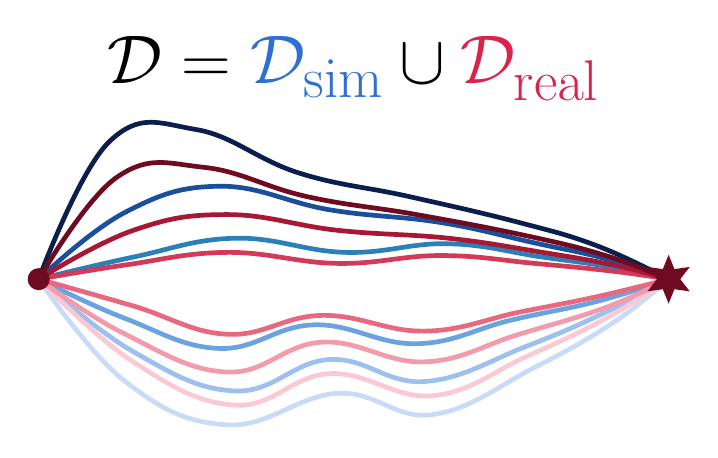
\begin{tikzpicture}[x=1cm,y=1cm,line cap=round,line join=round]

  % simulated rollouts (as in dataset_sim.tex)
  \begin{scope}[line width=1.7pt]
    \draw[sF] plot[smooth,tension=0.7] coordinates
      {(0,0) (1.1,-1.30) (2.4,-1.85) (3.8,-1.45) (5.0,-1.72) (6.3,-1.12) (7.3,-0.55) (8,0)};
    \draw[sE] plot[smooth,tension=0.7] coordinates
      {(0,0) (1.2,-0.92) (2.5,-1.42) (3.7,-1.02) (4.9,-1.30) (6.2,-0.85) (7.2,-0.42) (8,0)};
    \draw[sD] plot[smooth,tension=0.7] coordinates
      {(0,0) (1.1,-0.50) (2.3,-0.88) (3.5,-0.58) (4.8,-0.82) (6.0,-0.52) (7.1,-0.28) (8,0)};
    \draw[sC] plot[smooth,tension=0.7] coordinates
      {(0,0) (1.2,0.28) (2.5,0.52) (3.9,0.34) (5.2,0.45) (6.4,0.28) (7.3,0.15) (8,0)};
    \draw[sB] plot[smooth,tension=0.7] coordinates
      {(0,0) (1.1,0.85) (2.3,1.18) (3.7,0.88) (5.1,0.72) (6.3,0.46) (7.2,0.26) (8,0)};
    \draw[sA] plot[smooth,tension=0.7] coordinates
      {(0,0) (0.9,1.75) (2.0,1.90) (3.3,1.35) (4.7,1.05) (6.1,0.72) (7.1,0.42) (8,0)};
  \end{scope}

  % human-corrected real replays, interleaved with the simulated ones
  \begin{scope}[line width=1.7pt]
    \draw[rF] plot[smooth,tension=0.7] coordinates
      {(0,0) (1.2,-1.05) (2.5,-1.60) (3.7,-1.20) (5.0,-1.48) (6.2,-0.98) (7.2,-0.50) (8,0)};
    \draw[rE] plot[smooth,tension=0.7] coordinates
      {(0,0) (1.1,-0.70) (2.4,-1.18) (3.6,-0.80) (4.9,-1.05) (6.1,-0.70) (7.2,-0.36) (8,0)};
    \draw[rD] plot[smooth,tension=0.7] coordinates
      {(0,0) (1.2,-0.34) (2.4,-0.70) (3.6,-0.46) (4.9,-0.66) (6.1,-0.42) (7.1,-0.22) (8,0)};
    \draw[rC] plot[smooth,tension=0.7] coordinates
      {(0,0) (1.1,0.18) (2.4,0.34) (3.8,0.20) (5.1,0.30) (6.3,0.20) (7.3,0.10) (8,0)};
    \draw[rB] plot[smooth,tension=0.7] coordinates
      {(0,0) (1.2,0.62) (2.4,0.82) (3.8,0.62) (5.2,0.52) (6.4,0.34) (7.3,0.18) (8,0)};
    \draw[rA] plot[smooth,tension=0.7] coordinates
      {(0,0) (1.0,1.30) (2.1,1.42) (3.4,1.05) (4.8,0.82) (6.2,0.55) (7.2,0.30) (8,0)};
  \end{scope}

  \fill[rA] (0,0) circle (0.14);
  \node[star,star points=6,star point ratio=2.1,fill=rA,draw=none,
        minimum size=0.62cm,inner sep=0pt] at (8,0) {};

  % compile with \def\nolabel{} prepended for the curves-only version
  \ifx\nolabel\undefined
  \node[anchor=south] at (4,2.15)
    {\fontsize{30}{30}\selectfont $\mathcal{D}=
      \textcolor{simlbl}{\mathcal{D}_{\mathrm{sim}}}\cup
      \textcolor{reallbl}{\mathcal{D}_{\mathrm{real}}}$};
  \fi

\end{tikzpicture}
\end{document}
